\documentclass[10pt,a4paper]{article}

	\usepackage{amsmath,amssymb,amsthm,mathtools,amsfonts}
	\usepackage{breqn}
	\usepackage[utf8]{inputenc}
	\usepackage[english]{babel}
	\usepackage[T1]{fontenc}
	\usepackage{graphicx}
	\graphicspath{{../../img/}}

	%%%%%%%%%%%%%%%%%%%%%%%%%%%%%%%%%%%%%%%%%%%%%%%%%%%%%%%%%%%%%%%%%%%%%%%%%%%%%% Fonts

	\usepackage{fontspec}
	\setmainfont{Times New Roman}
	\newfontfamily\garamond[Numbers=OldStyle]{EB Garamond}
	\newfontfamily\plantin[Numbers=OldStyle]{Plantin MT Pro}
	\newfontfamily\wal{Walbaum Com}
	\newfontfamily\quotefont[Ligatures=TeX]{Linux Libertine O}
	\newfontfamily\vest{TRY Vesterbro Regular}
	\newfontfamily\vestb{TRY Vesterbro Poster}
	\newfontfamily\overp{Overpass}

	\newfontfamily\mysectionfont[Numbers=OldStyle]{Klavika light}

	\usepackage[pdfborder={0 0 0}]{hyperref}
	\usepackage{multicol}
	\usepackage{tabularx}
	\usepackage{enumitem}
	\usepackage{wrapfig}
		\setlength{\columnsep}{0pt}
		\setlength{\intextsep}{-10pt}
	\usepackage{caption}
	\usepackage[svgnames]{xcolor}
	\usepackage{dirtytalk}
	\usepackage[modulo]{lineno}
	\usepackage{hyperref}
	\usepackage{pdfpages}
	\usepackage{tasks}
	\newcommand\svar[1]{\newline\textcolor{red}{\textbf{Svar}\\#1}}
	\newcommand{\qm}[1]{``#1"}

	%%%%%%%%%%%%%%%%%%%%%%%%%%%%%%%%%%%%%%%%%%%%%%%%%%%%%%%%%%%%%%%%%%%%%%%%%%%%%% Colors

	\usepackage{xcolor}
	\usepackage{transparent}

	\definecolor{frbblue}{RGB}{47, 88, 109}
	\definecolor{hgred}{RGB}{140, 10, 10}
	\definecolor{frbgreenl}{RGB}{162, 202, 137}
	\definecolor{frbgreen}{RGB}{28, 85, 66}
	\definecolor{frbgrey}{RGB}{243, 245, 242}

	\usepackage{titlesec}
	\titleformat{\subsection}{\color{frbgreen}\overp\large}{}{}{}
	\newcommand{\source}[1]{Source: \href{#1}{#1}}
	\usepackage{lipsum}
	\usepackage{comment}
	\usepackage{ulem}

	\newcommand{\glos}[3]{\dotuline{#1}\marginpar{\scriptsize\textit{#3} #2}}

	\setlength{\parskip}{0.5\baselineskip}
	\setlength{\parindent}{0cm}
	\setlist[enumerate]{label=\alph*),left=20pt}

	\usepackage{titling}
	\setlength{\droptitle}{-12ex}
	\pretitle{\begin{center}\vestb\Huge\color{frbgreen}}
	\posttitle{\end{center}}
	\preauthor{\begin{center}\vest\Large\color{frbblue}}
	\postauthor{\end{center}}
	\predate{\begin{center}\vest}
	\postdate{\end{center}}

	\setcounter{secnumdepth}{0}

	\usepackage{tikz}

\begin{document}

\title{Eksamen S2601EnB}
\date{Sommer, 2026}
\author{Spørgsmål 7}
\maketitle

\begin{tikzpicture}[remember picture,overlay]
    \node[anchor=north east,yshift=-15pt,xshift=-45pt]%
       at (current page.north east)
        {
\includegraphics[scale=0.1]{frbvuc_logo.png}};
    \end{tikzpicture}

\thispagestyle{empty}

\vspace{-4em}

\begin{center}
{\color{frbblue}\rule{1\textwidth}{1pt}}
\end{center}

\subsection{Prøvemateriale}
\begin{description}
\item[Theme:] New Zealand
\item[Text:] Colleen Maria Lenihan, \qm{George Floyd: Whanganui café wouldn't let my Māori mum use the toilet}. Essay.

{[…] angiver forkortelser i forhold til originalen.}
\item[NS:] 2,9
\item[Instruction:] You must analyse and interpret \qm{George Floyd: Whanganui café wouldn't let my Māori mum use the toilet} and make a presentation (roughly 8 minutes) of the text and relate the text to the theme \qm{New Zealand}.

Apart from your own points, you must include the following points in your presentation:
  \begin{itemize}
\item Modes of appeal
\item Intention
\end{itemize}
\end{description}

\subsection{Bedømmelseskriterier, hf B}
Ved den \textbf{mundtlige prøve} lægges der vægt på, at eksaminanden
\begin{itemize}
  \item behersker et sammenhængende og forholdsvis flydende engelsk med relativ høj grad af grammatisk korrekthed
  \item giver en klart sammenhængende præsentation
  \item analyserer, fortolker og perspektiverer prøvematerialet med anvendelse af fagets analytiske begreber og metoder
  \item anvender den viden, der er opnået i arbejdet med det studerede emne.
\end{itemize}
Der lægges i bedømmelsen vægt på, at eksaminanden kan indgå i uddybende samtale om præsentationen.

Der gives én karakter ud fra en helhedsvurdering af eksaminandens præstation.


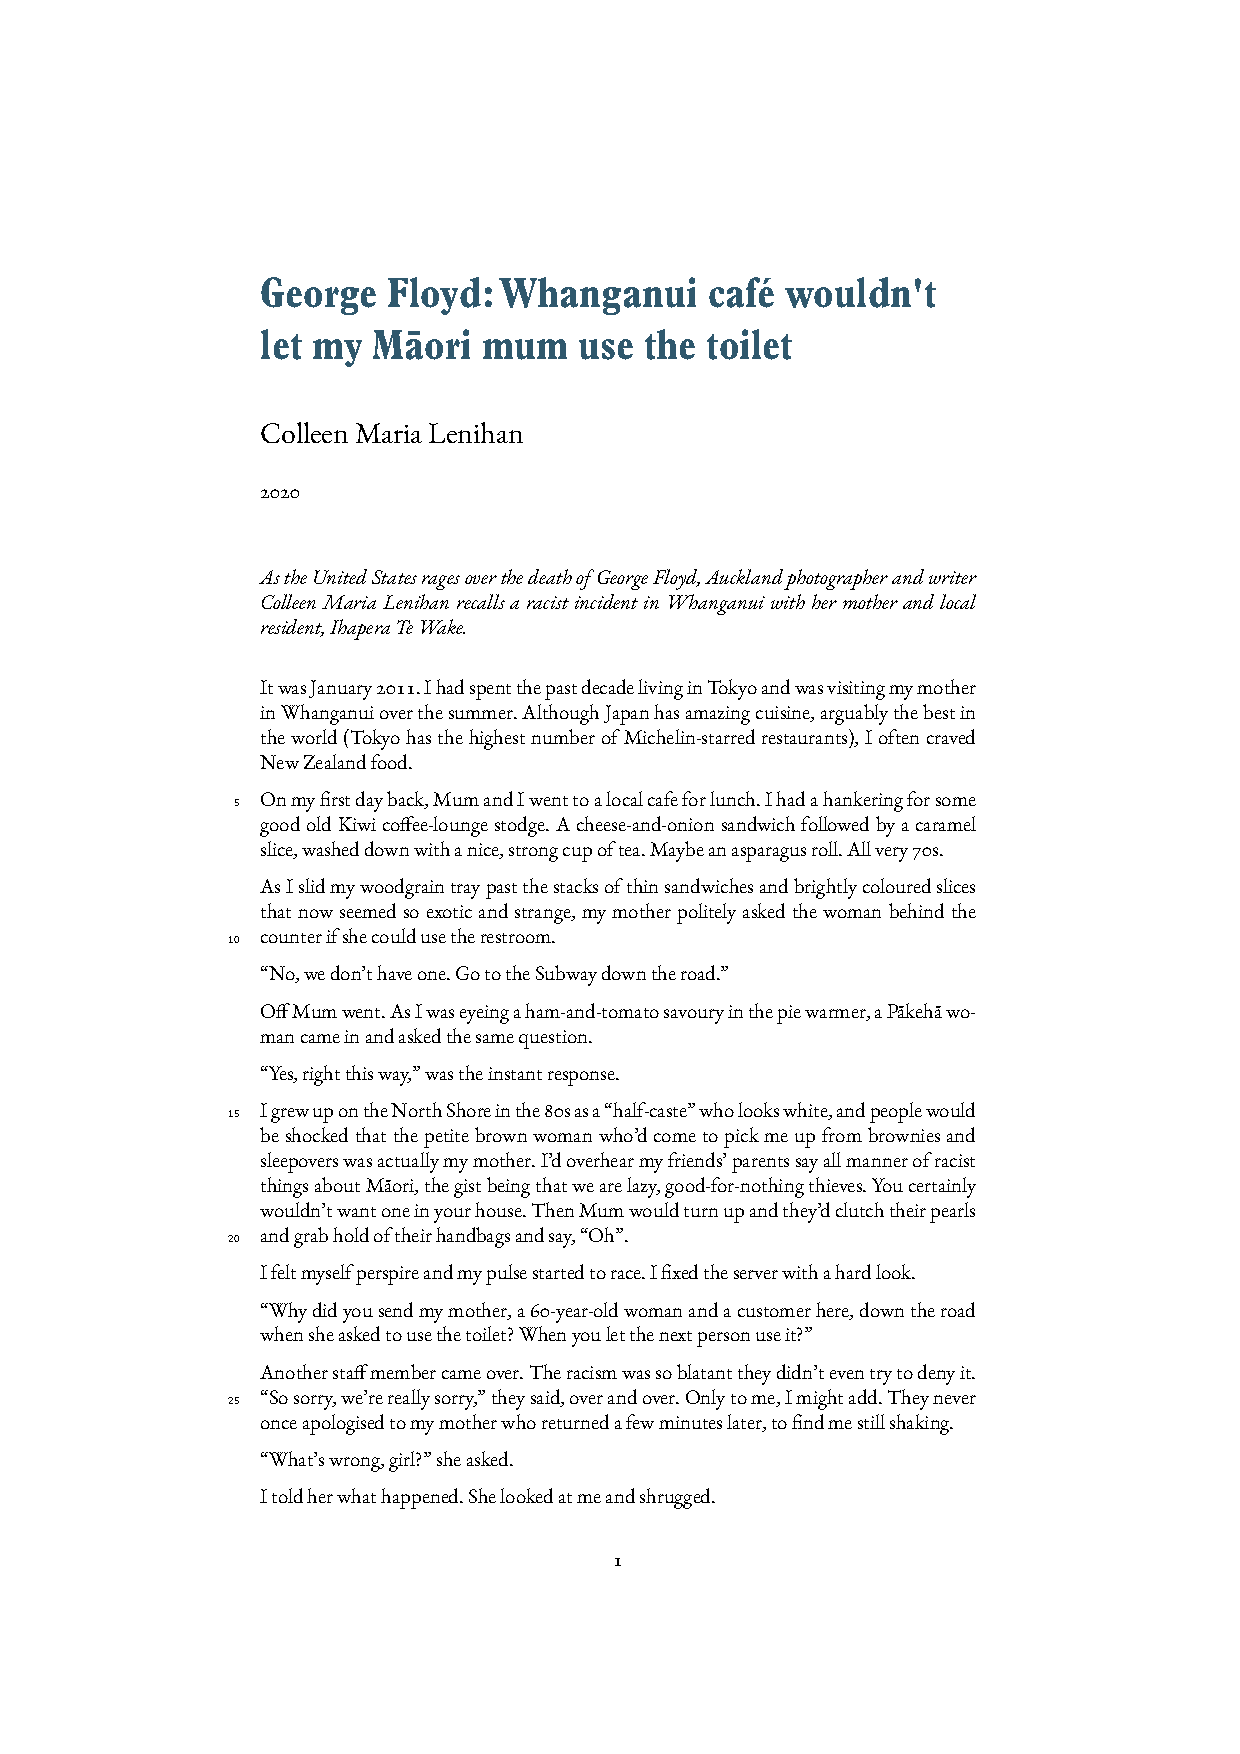
\includepdf[pages=1-]{./george_floyd.pdf}


\end{document}
